% =====================================================================
% Chapter I.1: What is a quantum field theory?
% =====================================================================
\section{What is a quantum field theory?}
\label{ch:what-is-qft}

There is a question that every course on quantum field theory postpones, and
that these notes take as their subject: what, exactly, \emph{is} a quantum field
theory? Not how to compute in one --- you know how to do that. You can
renormalize a loop integral, extract a cross section, run a coupling. The
question is what the object is that all this machinery computes \emph{about}.

For quantum mechanics the analogous question has an answer that fits on a
postcard. A quantum system is a Hilbert space $\mathcal{H}$, states are rays in
it, observables are self-adjoint operators, time evolution is a unitary
$e^{-iHt}$. Every textbook states these axioms in chapter one; nothing
discovered since 1930 has dislodged them. Now try to recall the corresponding
list from your quantum field theory course. There isn't one. What you were given
instead was a \emph{recipe} --- pick fields, write a Lagrangian, quantize,
renormalize --- together with the implicit promise that the recipe defines the
subject. The first purpose of this chapter is to show, by exhibiting concrete
and well-established physics, that it does not: there are quantum field theories
the recipe cannot produce, single theories it produces in several inequivalent
ways, and recipe-outputs that turn out not to exist. The second purpose is
constructive: to assemble the list of things a quantum field theory actually
provides --- its observables --- and to draw the picture that organizes
everything else in these notes, in which theories are points in a space, the
renormalization group is a flow on that space, and conformal field theories are
its fixed points.

\begin{qquestion}
What must we specify to specify a quantum field theory? And to what mathematical
and geometric objects does a quantum field theory, once specified, assign
physical data?
\end{qquestion}

\noin A warning about the spirit of what follows. Nothing in this chapter is a
complaint about the practical success of the standard framework, which is
the most quantitatively successful structure in the history of science and
which we will use constantly. The claim is about logic, not utility: the
standard framework is a description of how to \emph{present} certain
quantum field theories and expand them around free fields, and the subject
has outgrown the identification of theories with their presentations.
Making that distinction precise is worth a whole chapter, because almost
every modern development --- generalized symmetry, the bootstrap, duality,
the lattice--continuum program --- begins from it.

% =====================================================================
\subsection{The standard paradigm}
\label{sec:standard-paradigm}

Let us first state the inherited answer honestly, because it deserves it. The
textbook definition of a quantum field theory, circa 2000, is a procedure:

\begin{enumerate}
\item Choose fields: a collection of functions on spacetime transforming in
representations of the Poincar\'e group and of some internal (possibly gauge)
group.
\item Write the most general local Lagrangian density $\el[\phi, \partial\phi]$
consistent with the symmetries, keeping terms up to some power-counting
criterion (``renormalizability'').
\item Quantize: canonically, or via the path integral
\begin{equation}
Z = \int \de\phi \; e^{iS[\phi]}, \qquad S = \int d^dx \, \el ,
\label{eq:formal-pi}
\end{equation}
defined in practice by expanding around the Gaussian (free) theory.
\item Renormalize: absorb the divergences of the expansion into the couplings,
order by order.
\end{enumerate}

\noin The output of this procedure is a perturbation series for correlation
functions, and through the LSZ reduction formula, for scattering
amplitudes. The procedure's triumphs are not in dispute. Its flagship
number is the magnetic moment of the electron: the measured value $g/2 =
1.001\,159\,652\,180\,59\,(13)$ agrees with the Standard Model prediction
at the level of one part in $10^{12}$ --- the comparison is now limited by
independent measurements of $\alpha$, not by QFT itself.\footnote{Fan,
Myers, Sukra, Gabrielse, \texttt{2209.13084}, currently the most precisely
verified prediction in science. Seiberg's essay \emph{Thoughts About
Quantum Field Theory} opens with this number for the same rhetorical
purpose.} The same procedure, run in reverse by Wilson, explained why
critical exponents of fluids and magnets are computable at all. A
definition this successful does not get discarded; it gets
\emph{relocated}, and understanding where it belongs is the business of
Section~\ref{sec:theory-space}.

But look closely at what the procedure actually hands you. Step 3 writes down
the symbol \eqref{eq:formal-pi} and immediately retreats to an expansion around
the quadratic action. Each order of that expansion, after step 4, is finite and
unambiguous. The series as a whole is another matter, and here it pays to go to
the one spacetime where every step can be done exactly: a single point.

\begin{eexample}[The $\phi^4$ theory in zero dimensions]
\label{ex:zero-d}
Take spacetime to be a point. A ``field'' is then one real number $\phi$, the
``path integral'' is an ordinary integral, and the Euclidean $\phi^4$ partition
function is
\begin{equation}
Z(\lambda) = \frac{1}{\sqrt{2\pi}}\int_{-\infty}^{\infty} d\phi \;
  e^{-\frac{1}{2}\phi^2 - \frac{\lambda}{4!}\phi^4},
\label{eq:zerod-Z}
\end{equation}
normalized so that $Z(0) = 1$. There is nothing to renormalize and nothing to
gauge-fix; the entire content of ``quantizing the Lagrangian'' is this one
integral, which manifestly exists for all $\lambda \ge 0$.

Now run the textbook procedure: expand around the free theory. Exchanging the
sum with the integral,
\begin{equation}
Z_{\rm pert}(\lambda) = \sum_{n=0}^{\infty} \frac{1}{n!}
  \left(-\frac{\lambda}{4!}\right)^{\!n} \frac{1}{\sqrt{2\pi}}\int d\phi\;
  \phi^{4n} e^{-\frac{1}{2}\phi^2}
  = \sum_{n=0}^{\infty} a_n \lambda^n ,
\end{equation}
where the Gaussian moments are $(4n-1)!! = (4n)!/\big(2^{2n}(2n)!\big)$, so that
\begin{equation}
a_n = \frac{(-1)^n}{(4!)^n\, n!} \cdot \frac{(4n)!}{2^{2n}\,(2n)!}.
\label{eq:an}
\end{equation}
The first few terms, $Z_{\rm pert} = 1 - \frac{\lambda}{8} +
\frac{35\lambda^2}{384} - \cdots$, are exactly the sums of vacuum Feynman
diagrams with the usual symmetry factors. Up to this point, everything
matches the textbook treatment. But apply
Stirling's formula to \eqref{eq:an}:
\begin{equation}
|a_n| \;\sim\; \frac{1}{\pi n \sqrt{2}} \; n! \left(\frac{2}{3}\right)^{\!n}
\qquad (n \to \infty).
\label{eq:an-asymptotic}
\end{equation}
The coefficients grow \emph{factorially}: the ratio $|a_{n+1}/a_n| \approx
\tfrac{2}{3}n$ diverges, and the series has zero radius of convergence. For
\emph{no} value of $\lambda \neq 0$, however small, does the perturbative
expansion converge.

There is a beautifully physical way to see that this had to happen, due to
Dyson. Suppose the series converged in some disc $|\lambda| < R$. Then
$Z(\lambda)$ would be analytic at $\lambda = 0$ and in particular would exist
for small \emph{negative} $\lambda$. But at $\lambda < 0$ the integral
\eqref{eq:zerod-Z} diverges --- the potential is unbounded below, the theory has
no ground state --- so no such analytic continuation can exist, and $R =
0$.\footnote{Dyson's original argument (Phys.\ Rev.\ \textbf{85}, 631 (1952))
was made for QED, where it is heuristic; in zero dimensions it is a rigorous
one-line proof.}

The series is not useless --- it is \vocab{asymptotic}. Truncating at order $N$,
the error is controlled by the first omitted term, $|a_N \lambda^N| \sim
N!\,(2\lambda/3)^N$, which \emph{decreases} with $N$ until $N_\ast \approx
3/2\lambda$ and grows explosively afterwards. Truncating at the optimal order
leaves an irreducible error
\begin{equation}
\Delta Z \;\sim\; e^{-N_\ast} = e^{-3/2\lambda} ,
\label{eq:optimal-truncation}
\end{equation}
invisible at every finite order in $\lambda$. This is not a random number: the
action $S = \frac{1}{2}\phi^2 + \frac{\lambda}{4!}\phi^4$ has, besides $\phi =
0$, the complex saddle points $\phi_\ast^2 = -6/\lambda$ with $S(\phi_\ast) =
-3/2\lambda$, and it is these \emph{instanton-like} saddles that govern both the
large-order growth \eqref{eq:an-asymptotic} and the error
\eqref{eq:optimal-truncation}. Perturbation theory around one saddle knows about
the others only through the divergence of its own coefficients.
\end{eexample}

Three lessons, in increasing order of importance. First, the perturbation series
was never the theory: it is a particular asymptotic expansion \emph{of} the
theory, tied to a particular saddle point. Second, the theory exists anyway ---
here, trivially, as a convergent integral. Third, the gap between the two is
quantitative and structured: effects of order $e^{-3/2\lambda}$, the germ of
everything ``nonperturbative.'' In zero dimensions these statements are almost
embarrassing in their simplicity. Their force comes from the fact that they
persist in higher dimensions:
in $d > 0$ the same factorial growth afflicts the loop expansion of essentially
every interacting QFT, while the analogue of ``the integral exists anyway'' ---
some construction of the theory that does not lean on the expansion --- becomes
the entire problem. The recipe of steps 1--4 produces the series and is silent
about the object the series approximates.

\begin{reemark}[Borel resummation and resurgence]
\label{rem:borel}
For $\lambda > 0$ the zero-dimensional series can be completely repaired: its
Borel transform $B(t) = \sum_n a_n t^n / n!$ converges for $|t| < 3/2$ (the
singularity sits at $t = -3/2$, the instanton action again), and the Borel
integral $\int_0^\infty dt\, e^{-t} B(\lambda t)$ reproduces $Z(\lambda)$
exactly (Exercise~\ref{exr:borel}). The program of \emph{resurgence}
systematizes this: the perturbative series around each saddle encodes, through
the detailed structure of its divergence, the contributions of all the others.
In genuine QFTs the story is harder (renormalons join instantons among the Borel
singularities) and is an active subject; see Aniceto--Ba\c{s}ar--Schiappa
\arxiv{1802.10441} for a thorough introduction, and Part IV.5 for where it sits
today. We will not need resurgence machinery until then, but you should know
that ``the series diverges'' is the beginning of a theory, not the end of one.
\end{reemark}

One should be fair about what the old framework knows beyond the series. Lattice
regularization defines $Z$ nonperturbatively at finite cutoff, and constructive
field theory has \emph{proven} that interacting continuum limits exist in low
dimensions --- the $P(\phi)_2$ theories, $\phi^4_3$, Gross--Neveu$_2$,
Yukawa$_{2,3}$ all rigorously satisfy the Wightman axioms.\footnote{The
standard reference for the constructive program is Glimm--Jaffe,
\emph{Quantum Physics: A Functional Integral Point of View}; see also the
reading list at the end of this chapter.}
Instanton calculus patches in the leading $e^{-S_\ast}$ effects. The working
physicist's position circa 2000 --- ``the path integral means: lattice +
continuum limit, and perturbation theory is its asymptotic expansion'' --- is
coherent and, in its domain, correct. The trouble is the domain. The next
section presents four pieces of settled physics that fall outside it.

\begin{exercise}[easy]
\label{exr:an-check}
Verify $a_1 = -1/8$ and $a_2 = 35/384$ from \eqref{eq:an}, and check them
against the vacuum Feynman diagrams of $\phi^4$ theory (one and two vertices;
count symmetry factors). Then verify the asymptotic statement
\eqref{eq:an-asymptotic} numerically: compute $|a_{n+1}/a_n|$ for $n = 5, 10,
20$ and compare with $\tfrac{2}{3}(n + \tfrac{7}{4})$.
\hint{For the diagrams: at one vertex, the figure-eight has symmetry factor $8$.
For the ratio: use \eqref{eq:an} directly; no Stirling needed.}
\answ{$a_{n+1}/a_n = -\frac{(4n+4)(4n+3)(4n+2)(4n+1)}{24 \cdot 4 \cdot
(n+1)(2n+2)(2n+1)} = -\tfrac{2}{3}n - \tfrac{7}{6} + O(1/n)$, so the
quoted ratio is accurate to a few percent already at $n=10$.}
\end{exercise}

\begin{exercise}[classic]
\label{exr:dyson-qm}
(Dyson in quantum mechanics.) Consider the anharmonic oscillator $H =
\frac{1}{2}p^2 + \frac{1}{2}x^2 + \lambda x^4$. Adapt Dyson's argument to show
that the Rayleigh--Schr\"odinger series for the ground-state energy
$E_0(\lambda)$ must have zero radius of convergence. (Bender and Wu computed its
coefficients to high order in 1969 and found $|c_n| \sim n!\,3^n$, confirming
this.)
\hint{What happens to the spectrum of $H$ for $\lambda < 0$, no matter how
small? Think about tunneling out of the origin: the decay rate is $\sim
e^{-c/|\lambda|}$, which is non-analytic at $\lambda = 0$.}
\end{exercise}

\begin{exercise}[medium]
\label{exr:borel}
(Borel summation in $d=0$.) Define $B(t) = \sum_n a_n t^n/n!$ with $a_n$ as in
\eqref{eq:an}. Show that the series for $B$ converges for $|t| < 3/2$, and that
for $\lambda > 0$
\begin{equation*}
\int_0^\infty dt \, e^{-t}\, B(\lambda t) = Z(\lambda).
\end{equation*}
\hint{Insert $1 = \frac{1}{n!}\int_0^\infty dt\, e^{-t} t^n$ into the
(divergent) series for $Z$ and exchange sums and integrals where legal.
Convergence of $B$ follows from \eqref{eq:an-asymptotic}. The Borel
singularity at $t = -3/2$ sits on the \emph{negative} axis because the
series alternates --- this is why the integral along the positive axis is
safe. For $\lambda < 0$ the singularity obstructs the contour: the
ambiguity in avoiding it is $\sim e^{-3/2|\lambda|}$, the decay rate of
the metastable vacuum.}
\end{exercise}

% =====================================================================
\subsection{Four cracks}
\label{sec:four-cracks}

If the only deficiency of ``quantize a Lagrangian'' were the divergence of its
series, the fix would be technical and the old definition would stand. The
actual situation is more interesting: as physicists explored quantum field
theory away from weak coupling --- through supersymmetry, through string theory,
through the bootstrap, through rigorous statistical mechanics --- they found
that the map between Lagrangians and theories is neither surjective nor
injective, and in at least one textbook case not even well-defined. We present
four exhibits. None of them is derived here; each is a vignette with pointers to
the part of these notes where it is done properly, and to the literature. We
flag this clearly: \emph{in this section we cite, not derive} --- which is
itself a lesson in how this material is established.

\paragraph{Crack 1: a theory with no Lagrangian.}
There exists a six-dimensional interacting conformal field theory, the
\vocab{$(2,0)$ theory}, with the following r\'esum\'e. It was discovered in 1995 as
the decoupling limit of coincident M5-branes in M-theory, equivalently of type
IIB string theory on an A--D--E singularity.\footnote{Witten,
\texttt{hep-th/9507121}. The theory is labeled by an A--D--E Lie algebra;
``the'' $(2,0)$ theory of rank $N$ is the $A_{N-1}$ case.} It is, by every
available diagnostic, an honest local QFT: it has a stress tensor, local
operators with an operator product expansion, and correlation functions obeying
the usual axioms of conformal field theory. It is maximally supersymmetric, and
upon compactification on a circle it flows to five-dimensional Yang--Mills; on a
torus, to four-dimensional $\mathcal{N}=4$ Yang--Mills, whose S-duality becomes,
from six dimensions, the merely \emph{geometric} statement that a torus has a
modular group. And it has no Lagrangian --- not ``none found yet'' as a matter
of bookkeeping, but structurally: the theory has no coupling constant
whatsoever, no marginal or relevant deformation preserving its symmetry, hence
no dial to turn to reach weak coupling, hence nothing for a path-integral
expansion to expand around. Even the count of its degrees of freedom announces
the problem: anomaly and holographic computations show the number of degrees of
freedom of the rank-$N$ theory grows as $N^3$,\footnote{Henningson--Skenderis,
\texttt{hep-th/9806087}, from holography; Harvey--Minasian--Moore from anomaly
inflow. No free-field counting reproduces $N^3$.} a scaling no known collection
of free fields reproduces. Every property listed above was established through
string dualities and consistency arguments, not through any intrinsic
construction --- which is precisely the scandal. Compactifying the $(2,0)$
theory on Riemann surfaces generates the enormous ``class $\mathcal{S}$'' of
four-dimensional theories, most of which inherit its homelessness. The space of
quantum field theories is strictly larger than the space of Lagrangians. (Part
VI.4; Gaiotto \arxiv{0904.2715}, Tachikawa \arxiv{1312.2684}.)

\paragraph{Crack 2: one theory, several Lagrangians.}
The opposite failure is just as instructive: the map from Lagrangians to
theories is many-to-one, and not only in trivial ways (field redefinitions) but
in ways that exchange weak and strong coupling, bosons and fermions, gauge and
global. The cleanest examples live in 2+1 dimensions. Take the $O(2)$
Wilson--Fisher fixed point --- the critical point of a complex scalar with
$|\phi|^4$ interaction, the universality class of the superfluid transition in
$^4$He. \vocab{Particle--vortex duality} asserts that the very same conformal
field theory is reached by a \emph{different} Lagrangian: a complex scalar
coupled to a dynamical $U(1)$ gauge field (the abelian Higgs model), with the
global symmetry that counts particles on one side realized as the symmetry that
counts magnetic flux on the other,
\begin{equation}
|\partial_\mu \phi|^2 - |\phi|^4
\qquad \longleftrightarrow \qquad
|D_b \hat\phi|^2 - |\hat\phi|^4 + (\text{Maxwell for } b),
\label{eq:particle-vortex}
\end{equation}
both tuned to criticality.\footnote{Peskin (1978) and Dasgupta--Halperin (1981)
originally; stated in modern form, with the whole web it seeds, in
Seiberg--Senthil--Wang--Witten \arxiv{1606.01989}, whose \S1 is the recommended
first reading on what duality means.} Neither side is ``the'' description: the
elementary field of one is a topological soliton of the other. In 2016 this old
duality was joined by a \emph{seed} boson--fermion duality --- the gauged
Wilson--Fisher boson at Chern--Simons level one is a free Dirac fermion --- from
which a whole web of equivalences follows by formal gauging operations, with
experimental relevance from quantum Hall transitions to topological insulator
surfaces. If a single conformal field theory can be presented as bosons, as
gauged bosons, or as fermions, then asking ``which Lagrangian is the theory?''
is asking which coordinate chart is the manifold. (Part VI;
\arxiv{1606.01989}.)

\paragraph{Crack 3: computation without a Lagrangian.}
The cracks above could be dismissed as exotica --- supersymmetric,
low-dimensional. The third cannot, because it concerns the most pedestrian
strongly-coupled QFT in nature: the critical point of the three-dimensional
Ising model, the universality class of the liquid--vapor critical point and of
uniaxial magnets. The \vocab{conformal bootstrap} determines its low-lying
spectrum to stunning precision,
\begin{equation}
\Delta_\sigma = 0.5181489(10), \qquad \Delta_\epsilon = 1.412625(10).
\label{eq:ising-dims}
\end{equation}
These are the scaling dimensions that fix the classic critical exponents $\eta$
and $\nu$, and they are obtained using as input \emph{no Lagrangian, no lattice,
and no expansion parameter}: only unitarity, conformal symmetry, and the
associativity (crossing) of the operator algebra, implemented as a numerical
exclusion problem on the space of possible CFT data.\footnote{Numbers from
Poland--Rychkov--Vichi \arxiv{1805.04405}, Table II, obtained in Simmons-Duffin
\texttt{1612.08471}; the rigorous-island determinations are by
Kos--Poland--Simmons-Duffin--Vichi \texttt{1603.04436}. Rychkov--Su
\arxiv{2311.15844} reviews the current state of the art.} These values are more
precise than any Monte Carlo simulation of any lattice realization, and
incomparably more precise than the $\epsilon$-expansion applied to the $\phi^4$
Lagrangian that ostensibly ``defines'' the theory. Consistency conditions on the
observables, taken alone, pin the theory down: the observables behave as primary
data, the Lagrangian as one expendable presentation among several. How this is
possible --- why crossing plus unitarity is so much stronger than it looks ---
is the subject of Part III. (Part III.2; Rychkov's history \arxiv{2509.02779}
tells the remarkable story, from Polyakov's 1974 manifesto to the 2012 Ising
island.)

\paragraph{Crack 4: the Lagrangian that defines nothing.}
Finally, the recipe can fail at its own game. Its standard pedagogical example
--- the one in which every textbook teaches renormalization --- is $\phi^4$
theory in $d = 4$. In 2019 Aizenman and Duminil-Copin closed a forty-year-old
question by proving that the continuum limits of lattice $\phi^4_4$ and of the
4d Ising model, at or near criticality, are \emph{Gaussian}: every choice of
bare couplings, however strong, yields free fields when the cutoff is
removed.\footnote{Aizenman--Duminil-Copin \arxiv{1912.07973}. ``Marginal''
triviality: $d=4$ is the boundary case, where the proof requires a logarithmic
improvement over the classic tree-diagram bounds that settled $d \ge 5$ in the
1980s. This is a theorem of mathematics, not a scenario.} The interacting
continuum $\phi^4_4$ theory --- the object steps 1--4 purport to construct ---
does not exist. What does exist, and what the textbook computations were always
really about, is an \emph{effective} field theory with a finite cutoff, whose
couplings at low energy are insensitive to the details at the cutoff; this is
also the modern understanding of the Standard Model's scalar sector. Triviality
makes the relocation unavoidable: ``quantize this Lagrangian'' was never a
definition, but a procedure whose meaning depends on where in theory space you
stand and at what resolution you look. (Part VIII.5; the $d = 4-\epsilon$
Wilson--Fisher fixed point, which \emph{does} exist and explains why the recipe
works so well just below four dimensions, is constructed honestly in chapter
I.6.)

\medskip

\noin The four cracks share a single diagnosis. In each case the failure is not of quantum
field theory but of the identification of a theory with its presentation.
The $(2,0)$ theory has no presentation of Lagrangian type; the $O(2)$
fixed point has several; the 3d Ising CFT is best accessed with no
presentation at all; $\phi^4_4$ is a presentation of nothing. The
conclusion was stated by Polyakov already in 1974, in the introduction ---
it reads as a manifesto --- of the paper that founded the conformal
bootstrap: the description of a critical theory ``should be `democratic'
with respect to the different fields,'' i.e.\ should not privilege
whatever variables happen to appear in someone's bare
Hamiltonian.\footnote{Polyakov, \emph{Non-Hamiltonian approach to
conformal quantum field theory}, ZhETF \textbf{66} (1974) 23; quoted and
contextualized in Rychkov \arxiv{2509.02779}, \S5, which reproduces the
full passage. Seiberg's one-slide summary at the 2011 Solvay meeting ---
no Lagrangian for some theories, several for others, magic in amplitudes,
not mathematically rigorous --- is the same diagnosis a generation later.}

\begin{iidea}[A theory is its observables]
\label{idea:observables}
A quantum field theory is the total structure of its observables --- correlation
functions, spectra, partition functions, extended operators --- not any
particular procedure for generating them. Lagrangians, lattice models, bootstrap
data sets, and holographic duals are \vocab{presentations} of a theory:
coordinate descriptions, each with a domain of convenience, none privileged.
Some theories have many presentations; some have none we know.
\end{iidea}

This is the first organizing principle of these notes, and everything in this
part flows from taking it seriously. It immediately raises the question that the
rest of this chapter answers: if not a Lagrangian, then \emph{what}? What is the
structure that all presentations of a given theory present?

\begin{ppreview}[Where the cracks are repaired]
Theories without Lagrangians are constructed (by compactification and by
bootstrap) in Part VII.4 and Part III. Dualities are stress-tested and partially
derived in Part VI, with the tools --- symmetries, anomalies, line spectra ---
built in Part II. The bootstrap occupies Part III. Triviality, constructive
field theory, and the lattice--continuum dictionary occupy Part VIII. The
question ``what would a complete definition even look like?'' returns in Part
XII.1.
\end{ppreview}

\begin{exercise}[thinker]
\label{exr:duality-test}
Suppose a colleague proposes that two Lagrangians, like the two sides of
\eqref{eq:particle-vortex}, describe the same infrared theory. Neither side is
solvable. List every quantity you could in principle compare \emph{without}
solving either theory. (Symmetries? Their representations on local and extended
operators? Anomalies? Partition functions on nontrivial geometries? Behavior
under deformations?) Keep your list; Part II is the systematic theory of exactly
these duality invariants, and Part VI grades proposals against them.
\hint{The most useful invariants are the ones that cannot flow: discrete data,
quantized coefficients, anything protected under the renormalization
group. The modern checklist begins with the global symmetry
\emph{category} and its 't~Hooft anomalies.}
\end{exercise}

% =====================================================================
\subsection{What a quantum field theory assigns}
\label{sec:inventory}

If a theory is not its Lagrangian, our definition-shaped question has to be
approached from the other side: not ``what generates the theory?'' but ``what
does the theory \emph{provide}?'' Think of it as defining the species by its
behavior. Whatever a quantum field theory is, any presentation of it must
produce a definite collection of physical data, and two presentations describe
the same theory exactly when all of that data agrees. The modern consensus on
the inventory --- assembled from the axiomatic tradition and sharpened by the
functorial viewpoint --- is the following.\footnote{This is a physicist's
distillation of structures formalized, in different fragments, by the Wightman,
Osterwalder--Schrader, Haag--Kastler, and Atiyah--Segal axiom systems;
Section~\ref{sec:answer} below compares them. The geometric (``assign
data to manifolds'') formulation follows Segal, recently extended by
Kontsevich--Segal \arxiv{2105.10161}.}

\begin{ddefinition}[The inventory: data of a QFT]
\label{def:inventory}
A quantum field theory $\mathcal{T}$ in $d$ spacetime dimensions assigns:
\begin{enumerate}
\item to a closed $d$-dimensional spacetime $M_d$ (with metric, and possibly
other background fields): a \vocab{partition function}
$Z_{\mathcal{T}}[M_d] \in \complex$;
\item to points $x_1, \dots, x_n \in M_d$ decorated by labels $\op_1, \dots,
\op_n$ drawn from a set of \vocab{local operators}: correlation functions
$\langle \op_1(x_1) \cdots \op_n(x_n) \rangle_{M_d}$;
\item to a closed $(d-1)$-dimensional space $\Sigma_{d-1}$: a \vocab{Hilbert
space} $\mathcal{H}_{\Sigma}$ of states, with a $d$-manifold bounded by
$\Sigma$ defining a state in $\mathcal{H}_\Sigma$ (cutting and gluing);
\item to closed submanifolds of intermediate dimension, decorated by labels from
sets of \vocab{extended operators} (line operators, surface operators, \dots),
and to boundaries and interfaces: correlation functions in their presence;
\end{enumerate}
subject to consistency conditions --- locality of the operators, compatibility
of cutting and gluing, unitarity/reflection positivity, convergence structures
for the operator product expansion --- that subsequent chapters make precise.
\end{ddefinition}

Each entry of the inventory gets a chapter of its own (local operators in I.2,
extended operators in I.3, states and gluing in I.4), so here we stay at the
level of orientation, and the orientation is best gained by noticing what the
list does \emph{not} contain. There are no fields: ``$\phi$'' appears nowhere,
only the operators $\op_i$, and dualities like \eqref{eq:particle-vortex} show
that what one presentation calls an elementary field another calls a composite
or a soliton. There is no Lagrangian and no gauge group --- the gauge
``symmetry'' of the abelian Higgs side of \eqref{eq:particle-vortex} is
invisible in the inventory, a redundancy of that presentation rather than a
property of the theory (a point developed carefully in Part V.1). And there are
no particles: particles are states in $\mathcal{H}$ that happen to organize
themselves into asymptotic excitations when the theory is gapped, an excellent
emergent concept in some theories and simply absent in others (a conformal
theory like 3d Ising has a continuous spectrum of scaling states and no
particles at all). Item 4 --- defects --- would not have appeared on anyone's
list in 2000 and is the most consequential modern addition: theories with
identical local correlators can differ in their extended operators, so the
extended sector is part of the \emph{definition}, not a garnish. That lesson
gets chapter I.3 to itself.

The right way to internalize the inventory is to watch all of it materialize in
a system so small that nothing can hide. Quantum mechanics is a quantum field
theory in $d = 1$ --- the ``fields'' are functions of time only --- and one
particular quantum mechanics is, for reasons that will keep paying off through
Part V, an ideal specimen for the purpose.

\begin{eexample}[The inventory in $d=1$: a particle on a circle]
\label{ex:particle-circle}
Take a free particle of unit mass on a circle, $q \simeq q + 2\pi$, with
Lorentzian Lagrangian
\begin{equation}
L = \frac{1}{2}\dot q^2 + \frac{\theta}{2\pi} \dot q .
\label{eq:circle-lagrangian}
\end{equation}
The second term is our first \vocab{topological term}: a total derivative, with
no effect on the equations of motion, whose coefficient $\theta$ will
nonetheless turn out to be physical --- the one-dimensional ancestor of the
$\theta$-angles of Yang--Mills theory.\footnote{This example is worked out, as a
warm-up for 4d gauge theory, in Gaiotto--Kapustin--Komargodski--Seiberg
\arxiv{1703.00501}, Appendix D.1, whose conventions we follow. It reappears in
C\'ordova--Freed--Lam--Seiberg \arxiv{1905.09315} as the simplest anomaly in
parameter space.}

\emph{The Hamiltonian presentation.} The momentum conjugate to $q$ is $\Pi =
\dot q + \frac{\theta}{2\pi}$, and the Hamiltonian is
\begin{equation}
H = \frac{1}{2}\Big(\Pi - \frac{\theta}{2\pi}\Big)^2 .
\end{equation}
The inventory begins to fill in. \emph{States} (item 3): space is a point, and
the Hilbert space assigned to it is $\mathcal{H} = L^2(S^1)$, spanned by
$\braket{q}{n} = e^{inq}/\sqrt{2\pi}$ with $n \in \ints$ --- single-valuedness
of the wavefunction quantizes $\Pi$ to integers. The spectrum is
\begin{equation}
E_n = \frac{1}{2}\Big(n - \frac{\theta}{2\pi}\Big)^2 .
\label{eq:circle-spectrum}
\end{equation}
\emph{Local operators} (item 2): the well-defined operators are built from
$e^{\pm iq}$ and $\Pi$ ($q$ itself is not single-valued, hence not an operator
--- already a hint that ``the field'' is not sacred), with correlators like
$\bra{0} e^{iq(t)} e^{-iq(0)} \ket{0}$ computable by inserting energy
eigenstates. \emph{Partition function} (item 1): the closed $1$-manifold is a
circle; continuing to Euclidean time and traversing a circle of circumference
$\beta$,
\begin{equation}
Z(\beta, \theta) = \tr e^{-\beta H}
  = \sum_{n \in \ints}
    \exp\left[-\frac{\beta}{2}\Big(n - \frac{\theta}{2\pi}\Big)^2\right].
\label{eq:Z-hamiltonian}
\end{equation}

Two features of the spectrum \eqref{eq:circle-spectrum} repay a hard look.
First, \emph{$\theta$ is an angle}: $\theta \to \theta + 2\pi$ shifts $n \to
n+1$ and leaves the spectrum --- and every entry of the inventory --- invariant.
(Operatorially, $H_{\theta+2\pi} = e^{iq} H_\theta e^{-iq}$.) Second, the
invariance is realized \emph{nontrivially}: as $\theta$ runs from $0$ to $2\pi$
the levels cross, and at exactly $\theta = \pi$ the ground state is two-fold
degenerate, $E_0 = E_1$. A total-derivative coupling has produced physical
consequences, periodic in $2\pi$, with a level crossing at the symmetric point
that --- as we will see in Parts II.7 and V.3 --- no deformation respecting the
symmetries can remove. This is the entire conceptual skeleton of ``Yang--Mills
at $\theta = \pi$,'' in a system solvable by inspection.

\emph{The path-integral presentation.} Now compute $Z(\beta,\theta)$ the other
way, as a sum over all maps from the Euclidean time circle to the target circle.
Such maps fall into disconnected topological classes labeled by the
\vocab{winding number} $w \in \ints$; in each class the topological term
contributes the \emph{phase} $e^{i\theta w}$ --- topological terms acquire no
factor of $i$ under Wick rotation and remain imaginary in Euclidean signature
(Appendix~\ref{app:conventions}; this is the single most common sign error in
the subject). The action in the class $w$ is minimized by $q_w(\tau) = 2\pi w
\tau/\beta$, with $S_{\rm E}[q_w] = 2\pi^2 w^2/\beta$, and the Gaussian
fluctuations around $q_w$ are $w$-independent, contributing the free-particle
factor $\sqrt{2\pi/\beta}$ (Exercise~\ref{exr:fluctuation}). Hence
\begin{equation}
Z(\beta,\theta) = \sqrt{\frac{2\pi}{\beta}} \sum_{w \in \ints}
  \exp\left[-\frac{2\pi^2 w^2}{\beta} + i \theta w\right].
\label{eq:Z-winding}
\end{equation}
Expressions \eqref{eq:Z-hamiltonian} and \eqref{eq:Z-winding} look nothing alike
--- one is a sum over momenta with $\theta$ in the exponents' shifts, the other
a sum over windings with $\theta$ as a phase --- yet they are equal, exactly, by
the Poisson resummation formula $\sum_n f(n) = \sum_w \hat f(2\pi w)$ applied to
the Gaussian (Exercise~\ref{exr:poisson}). They are two presentations of one
theory, and they are useful in opposite regimes: at low temperature ($\beta \to
\infty$) the Hamiltonian sum is dominated by its first term or two while the
winding sum converges slowly, and at high temperature ($\beta \to 0$) the roles
reverse. This small duality is worth remembering as a template: the same
observable admits two expansions, each accurate in the regime where the
other fails. Part VII is devoted to this phenomenon in quantum field theory
proper.
\end{eexample}

The example is humble, but every theme of this chapter is present in it: data
assigned to geometric objects (a Hilbert space to a point, a number to a
circle); operators defined by the theory rather than by the classical
configuration space ($e^{iq}$, not $q$); a parameter space with nontrivial
topology ($\theta \in S^1$) and physics pinned to its special points; and two
presentations related by a nontrivial identity. When in later chapters the going
gets abstract, return here.

There is one more thing the example quietly demonstrates: at $\theta = \pi$ the
classical symmetry $C: q \to -q$ combines with the shift symmetry of the free
particle into a group that is realized on $\mathcal{H}$ only \emph{projectively}
--- the operators implementing it commute only up to a phase. The two-fold
degeneracy is the direct consequence, and the projective phase is the simplest
example of a \vocab{'t~Hooft anomaly}, the exactly-conserved quantity of the
renormalization group that Part II builds into the subject's sharpest
tool.\footnote{GKKS \arxiv{1703.00501}, eqs.\ (D.5)--(D.10): the symmetry group
at $\theta=\pi$ is a central extension of $O(2)$ --- $\mathrm{Pin}(2)$ --- and a
$\mathrm{Pin}(2)$ that cannot be reduced to $O(2)$ forces degenerate pairs.} We
flag it and move on; it returns in II.7 with the machinery to do it justice.

\begin{exercise}[easy]
\label{exr:theta-periodicity}
Show directly that $U = e^{iq}$ is a well-defined unitary operator on
$L^2(S^1)$, that $U H_\theta U^\dagger = H_{\theta + 2\pi}$, and that $U$ maps
$\ket{n} \to \ket{n+1}$. Conclude that all inventory data is $2\pi$-periodic in
$\theta$, and identify which states cross at $\theta = \pi$.
\hint{Work in the $\ket{n}$ basis throughout; $e^{iq}$ is a shift operator on
momentum eigenstates.}
\end{exercise}

\begin{exercise}[classic]
\label{exr:poisson}
Prove the Poisson resummation formula $\sum_{n \in \ints} f(n) =
\sum_{w\in\ints} \hat f(2\pi w)$, $\hat f(k) = \int dx\, f(x) e^{-ikx}$, and use
it to derive \eqref{eq:Z-winding} from \eqref{eq:Z-hamiltonian}, including the
prefactor and the sign of the phase.
\hint{The Dirac comb $\sum_n \delta(x - n)$ is periodic, so it equals its own
Fourier series; integrate $f$ against both expressions. For the
application: complete the square in \eqref{eq:Z-hamiltonian} first.}
\answ{With $f(x) = e^{-\frac{\beta}{2}(x - \frac{\theta}{2\pi})^2}$ one finds
$\hat f(2\pi w) = \sqrt{2\pi/\beta}\; e^{-2\pi^2 w^2/\beta}\, e^{-i\theta
w}$; relabeling $w \to -w$ gives \eqref{eq:Z-winding}.}
\end{exercise}

\begin{exercise}[medium]
\label{exr:fluctuation}
Justify the prefactor in \eqref{eq:Z-winding}: show that the Gaussian integral
over periodic fluctuations $\delta q(\tau)$ around any winding saddle is
independent of $w$, and that the zero mode (the constant shift of $q$) produces
a factor of the target-circle circumference, yielding in total the free-particle
result $2\pi/\sqrt{2\pi\beta} = \sqrt{2\pi/\beta}$.
\hint{$S_{\rm E}[q_w + \delta q] = S_{\rm E}[q_w] + \frac{1}{2}\int \dot{\delta
q}^2$ exactly --- the action is quadratic and the cross term integrates to
zero by periodicity. For the normalization, compare with the diagonal heat
kernel of a free particle on a line, $\bra{q}e^{-\beta H}\ket{q} =
1/\sqrt{2\pi \beta}$.}
\end{exercise}

\medskip
The particle on a circle entered through a Lagrangian, however --- hardly a
clean break from the old paradigm. So let us fill the same inventory from the
opposite end of physics: a statistical lattice with no Lagrangian, no continuum,
and at first sight no quantum mechanics at all.

\begin{eexample}[The Ising chain, read as a field theory]
\label{ex:ising-chain}
Put classical spins $s_i = \pm 1$ on $N$ sites of a periodic chain, with energy
favoring alignment, and define
\begin{equation}
Z_N = \sum_{\{s_i = \pm 1\}} \, \prod_{i=1}^{N} e^{J s_i s_{i+1}} ,
  \qquad s_{N+1} \equiv s_1 ,
\label{eq:ising-Z}
\end{equation}
where $J > 0$ absorbs the temperature. This is a Euclidean QFT presentation in
which spacetime itself is discrete: the chain is a one-dimensional
``spacetime,'' \eqref{eq:ising-Z} its partition function on a (discrete) circle.

The structure of the inventory emerges from a single move. Define the $2\times
2$ \vocab{transfer matrix} with entries $T_{s s'} = e^{J s s'}$,
\begin{equation}
T = \begin{pmatrix} e^{J} & e^{-J} \\ e^{-J} & e^{J} \end{pmatrix}
= e^{J}\,I + e^{-J} \sigma_x ,
\qquad \text{eigenvalues} \quad \lambda_\pm = 2\cosh J,\; 2 \sinh J .
\end{equation}
Multiplying along the chain and summing over spins,
\begin{equation}
Z_N = \tr \, T^N = \lambda_+^N + \lambda_-^N .
\label{eq:ising-trace}
\end{equation}
Compare item by item with the previous example. The \emph{Hilbert space}
assigned to a slice of this spacetime --- a single site --- is $\complex^2$, the
span of $\ket{\uparrow}, \ket{\downarrow}$. The \emph{Euclidean time evolution}
over one lattice step is $T$, the discrete stand-in for $e^{-aH}$. The
\emph{partition function on a circle} is a trace, exactly as $\tr e^{-\beta H}$
was. And the \emph{correlators}: inserting $\sigma_z$ at sites $0$ and $r$,
\begin{equation}
\langle s_0 s_r \rangle = \frac{\tr \left( \sigma_z T^{r} \sigma_z T^{N-r}
\right)}{\tr T^N}
\;\xrightarrow{\;N \to \infty\;}\;
\left(\frac{\lambda_-}{\lambda_+}\right)^{\!r} = (\tanh J)^r = e^{-r/\xi},
\label{eq:ising-correlator}
\end{equation}
with \vocab{correlation length} $\xi = 1/\ln \coth J$
(Exercise~\ref{exr:ising-correlator}). Two general morals hide in this formula.
The correlation length is the inverse of the \emph{gap}: $1/\xi =
\ln(\lambda_+/\lambda_-)$ is the spacing of the transfer matrix's spectrum, the
discrete avatar of $m = E_1 - E_0$. And \vocab{cluster decomposition} ---
correlations factorize at long distance, $\langle s_0 s_r \rangle \to \langle s
\rangle^2$ --- is on explicit display: it is nothing but the statement that the
largest eigenvalue dominates.

Now take the \emph{continuum limit}, the move that will occupy all of Part VIII;
here it can be done exactly. Give the lattice a physical spacing $a$ and send $a
\to 0$, $N \to \infty$. For the limit to retain any physics, the correlation
length \emph{in lattice units} must diverge, so $J \to \infty$ too; the
combination to hold fixed is the physical gap. Writing $T = e^J\big(I +
e^{-2J}\sigma_x + \cdots\big)$ and matching to $T \simeq e^{-aH +
\text{const}}$,
\begin{equation}
H = -\Gamma \sigma_x , \qquad \Gamma = \frac{e^{-2J}}{a} \;\; \text{held fixed
as } a \to 0 .
\label{eq:ising-continuum}
\end{equation}
The continuum limit of the classical Ising chain is the quantum mechanics of a
single spin in a transverse field --- Hilbert space $\complex^2$, gap $2\Gamma$,
physical correlation length $\xi_{\rm phys} = a\,\xi \to 1/2\Gamma$. Every
microscopic detail (the lattice, the specific nearest-neighbor form, corrections
to the exponentiation) has washed out into one parameter. This is
\vocab{universality} in its simplest instance, and it is the mechanism that makes
``QFT from a lattice'' meaningful at all: the continuum theory remembers only
the data that survives the limit.
\end{eexample}

Two systems could hardly look more different than a quantum particle on a circle
and a classical chain of spins, yet they filled the same inventory in the same
pattern: Hilbert space on a slice, (Euclidean) evolution operator, trace on a
circle, correlators with definite decay. That pattern --- not any Lagrangian ---
is what Definition~\ref{def:inventory} axiomatizes. The chain also displays, in
miniature, the claim from the chapter opening that the standard paradigm gets
\emph{relocated} rather than discarded: ``quantize a Lagrangian'' lives inside
the inventory picture as one family of presentations (start from classical
configurations, build $T$ or $e^{iS}$, read off the data), valid whenever it
converges on something --- and the chain shows there are presentations,
perfectly good ones, that never mention a classical action in the continuum.

One disclaimer, before the lattice picture settles in too comfortably as ``the''
nonperturbative definition. In $d = 1$ the continuum limit
\eqref{eq:ising-continuum} is a theorem of elementary analysis. In higher
dimensions, ``the continuum limit exists and is universal'' is a theorem only in
special cases, a well-supported conjecture in most, and --- this is the surprise
of the 2020s --- \emph{false} in instructive ones, where lattice models produce
continuum descriptions that violate cherished axioms (fractons, Part VIII.4) or
where the limit exists but is free despite all appearances (triviality, crack
4). The lattice is a presentation too, with its own dictionary problems; Part
VIII is the audit.

\begin{exercise}[easy]
\label{exr:ising-field}
Add a magnetic field: $Z_N = \sum_{\{s\}} e^{\sum_i (J s_i s_{i+1} + h s_i)}$.
Find the symmetric transfer matrix, its eigenvalues, and the magnetization $m =
\langle s_i \rangle$ in the thermodynamic limit.
\hint{Use $T_{ss'} = e^{J s s' + \frac{h}{2}(s + s')}$ to keep $T$ symmetric.
Then $m = \partial \ln\lambda_+ /\partial h$ at fixed $J$.}
\answ{$\lambda_\pm = e^J \cosh h \pm \sqrt{e^{2J} \sinh^2 h + e^{-2J}}$, giving
$m = \sinh h / \sqrt{\sinh^2 h + e^{-4J}}$: smooth for every $J < \infty$,
with no spontaneous magnetization at $h = 0$.}
\end{exercise}

\begin{exercise}[classic]
\label{exr:ising-correlator}
Derive \eqref{eq:ising-correlator}: insert $\sigma_z$ operators into the trace,
evaluate in the eigenbasis of $T$, and keep track of the finite-$N$ corrections.
Verify cluster decomposition and extract $\xi$.
\hint{$\sigma_z$ is off-diagonal in the eigenbasis $\ket{\pm} = (\ket{\uparrow}
\pm \ket{\downarrow})/\sqrt 2$: $\sigma_z \ket{\pm} = \ket{\mp}$. The
exact answer is $\big(\lambda_+^{N-r}\lambda_-^{r} +
\lambda_-^{N-r}\lambda_+^{r}\big)/\big(\lambda_+^N + \lambda_-^N\big)$.}
\end{exercise}

\begin{exercise}[medium]
\label{exr:ising-continuum}
Make the continuum limit \eqref{eq:ising-continuum} precise. Show that the
corrections to $T \approx e^{J} e^{-aH}$ are of relative order $e^{-4J} =
(a\Gamma)^2$ and hence vanish in the limit; show that the limit of $N$-site
quantities with $Na = \beta_{\rm phys}$ fixed reproduces the spin-$\tfrac12$
thermal traces; and verify $\xi_{\rm phys} \to 1/2\Gamma$ from
\eqref{eq:ising-correlator}.
\end{exercise}

\begin{exercise}[thinker]
\label{exr:no-transition}
The chain never orders: Exercise~\ref{exr:ising-field} shows the free energy is
analytic in $(J, h)$ for all finite $J$. Give two proofs that no phase
transition can occur in the 1d Ising model with short-range interactions: (a)
algebraic --- the transfer matrix has strictly positive entries; invoke the
Perron--Frobenius theorem to show $\lambda_+ > \lambda_-$ always, so the gap
never closes; (b) physical --- estimate the free energy of a single domain wall
in a chain of length $L$ and show entropy always wins (Peierls' argument, run in
reverse). What do these arguments use about $d = 1$, and which step fails in $d
= 2$?
\hint{For (b): a wall costs fixed energy $2J$ but can sit at any of $\sim L$
positions, so $\Delta F = 2J - T\ln L \to -\infty$. In $d=2$ a wall is a
line whose energy \emph{and} entropy both scale with its length --- the
competition becomes a genuine fight, and Peierls showed order wins at low
temperature.}
\end{exercise}

% =====================================================================
\subsection{Locality, the one non-negotiable}
\label{sec:locality}

The inventory of Definition~\ref{def:inventory}, as stated, is satisfied by
systems nobody would call a field theory --- nothing yet distinguishes the Ising
chain from a quantum computer's register or from a single harmonic oscillator,
which also assigns Hilbert spaces and thermal traces. What makes a theory a
theory \emph{of fields} is not the size of its Hilbert space but the way its
observables are organized by \emph{geometry}: degrees of freedom are distributed
over space, and they interact only with their neighbors. Every word of ``quantum
field theory'' except ``locality'' is negotiable --- we have already negotiated
away the fields --- and the modern attitude is to treat locality as the actual
subject. QFT is what you get when many degrees of freedom are organized locally;
everything else is presentation.

This one idea wears different uniforms in different formulations, and learning
to recognize it in all of them is part of the training:

\begin{itemize}
\item \emph{In the operator content}: operators are labeled by the points (and
submanifolds) where they live, and the product of two nearby local operators is
again a local operator --- the \vocab{operator product expansion}, the subject of
chapter I.2.
\item \emph{In Lorentzian signature}: measurements at spacelike separation are
independent,
\begin{equation*}
[\op_1(x), \op_2(y)] = 0 \qquad \text{for } (x-y)^2 > 0,
\end{equation*}
the statement of \vocab{microcausality} (Exercise~\ref{exr:microcausality}).
\item \emph{In Euclidean correlators}: \vocab{cluster decomposition}, already
met in \eqref{eq:ising-correlator} --- distant regions decorrelate.
\item \emph{In the dynamics}: the Hamiltonian is an integral of a local density.
Better, because it is presentation-independent: the theory possesses a local
\vocab{stress tensor} $T_{\mu\nu}(x)$ --- the operator that measures energy and
momentum density, and the response of the theory to deforming the geometry it
lives on. The stress tensor is the one operator every local QFT shares, and its
existence is the sharpest single criterion for ``is this a local field theory?''
(Chapter I.2 develops it; Part X makes it the protagonist.)
\item \emph{In the path integral and on the lattice}: the action/energy is a sum
of terms each involving only nearby points --- nearest-neighbor couplings in
\eqref{eq:ising-Z} --- which is what makes \emph{cutting} spacetime along a slice
meaningful and gives the gluing rules of item 3 of the inventory their content
(chapter I.4).
\end{itemize}

\noin These are not independent axioms but facets of one property, and their
precise interrelation (which implies which, under what hypotheses) is
genuinely subtle --- it is the content of the reconstruction theorems
discussed in chapter I.2. For orientation, the slogan suffices:

\begin{iidea}[Locality is the subject]
\label{idea:locality}
A quantum field theory is a quantum system whose observables are organized by
the geometry of spacetime, with independence at large separation and a local
stress tensor as the operator witness. Locality is the one ingredient of the
textbook definition that survives unweakened into every modern formulation ---
and the boundary of QFT as a subject traces exactly where locality starts to
fail.
\end{iidea}

The final clause matters because the failure modes of locality are themselves
instructive. A
quantum system with all-to-all couplings --- mean-field models, or the SYK model
beloved of holographers --- has no notion of spatial distance and is quantum
mechanics, not field theory (often a useful caricature of one, which is its
point). More exotically, the \emph{little string theories} arising on NS5-branes
have local energy \emph{density} in a loose sense but provably no stress tensor
and no local operators creating their excitations; they sit just outside the
boundary, and Part XII.3 visits them as instructive aliens. And systems with
power-law interactions, like the long-range Ising model $J_{ij} \sim
|i-j|^{-1-s}$, interpolate: for $s$ large enough they flow to ordinary local
field theories, for small $s$ to genuinely nonlocal continuum theories, with a
phase boundary in between --- locality of the IR theory is itself a dynamical
question.

\begin{nnote}
Locality should not be confused with \emph{Lorentz invariance}, its frequent
companion. Nonrelativistic, anisotropic, and Lifshitz-type field theories are
perfectly local, organized by geometry, and within our subject (condensed matter
supplies them in bulk); they simply weight time and space asymmetrically. The
axiom systems of Section~\ref{sec:answer}, built around the Poincar\'e group,
mostly exclude them --- one of several signs that the existing axioms draw the
boundary in the wrong place. Fractons (Part VIII.4) push on exactly this seam.
\end{nnote}

Why promote locality, rather than, say, unitarity or symmetry, to the
definition's one fixed point? Because locality is what gives quantum field
theory its unreasonable universality --- the empirical fact, which the next
section turns into a picture, that the same continuum theories appear as
descriptions of magnets, fluids, metals, the QCD vacuum, and the early universe.
The mechanism is the renormalization group: whatever the microscopic degrees of
freedom, so long as they are many and locally coupled, viewing them at longer
and longer wavelengths erases microscopic detail in a controlled way, and the
possible long-distance destinations are heavily constrained precisely
\emph{because} locality survives the coarse-graining. Wilson's insight, restated
in the vocabulary of this chapter: QFT is not fundamentally a theory of
elementary particles; it is the universal effective description of
locally-organized many-body systems, of which elementary particle physics is one
(spectacular) instance.\footnote{Seiberg's \emph{Thoughts About QFT} presses
this point: ``quantum field theory is the modern calculus --- the natural
language for describing diverse phenomena.'' The high-energy and
condensed-matter views of what a QFT is are compared, as two charts on one space
of theories, in Section~\ref{sec:theory-space}.}

\begin{exercise}[classic]
\label{exr:microcausality}
(Microcausality for the free scalar.) In the free massive scalar theory in $d=4$
with mostly-plus signature, the commutator of fields is a c-number, $[\phi(x),
\phi(y)] = \Delta(x-y)\,I$. Compute $\Delta$ from the mode expansion
and prove it vanishes whenever $x - y$ is spacelike.
\hint{$\Delta(x-y) = \int \frac{d^3p}{(2\pi)^3 2E_p} \big( e^{ip\cdot(x-y)} -
e^{-ip\cdot(x-y)} \big)$ with $p \cdot x = -E t + \mathbf{p} \cdot \mathbf{x}$ in
mostly-plus. For spacelike separation there is a Lorentz frame with $x^0 =
y^0$; show the integrand is then odd under $\mathbf{p} \to -\mathbf{p}$. Why does
this argument fail (as it must) for timelike separation?}
\end{exercise}

% =====================================================================
\subsection{Theory space: the picture to keep}
\label{sec:theory-space}

We can now assemble the chapter's deliverable: the picture within which all
twelve parts of these notes take place. It needs three ingredients, all already
on the table --- the inventory (a theory is a consistent assignment of
observables), locality (the assignment is organized by geometry), and
universality (microscopically different systems share long-distance
descriptions).

Imagine, then, the set of all quantum field theories in $d$ dimensions: every
consistent inventory, whether or not anyone has presented it. Call it
\vocab{theory space}. A point of theory space is a theory --- the 3d Ising CFT
is a point, the free photon is a point, QCD with physical quark masses is a
point. A Lagrangian is not a point: it is a \emph{name} for a point (and
dualities are the statement that points have several names). This space is the
arena. Its geography is given by the \vocab{renormalization group}: inspecting a
theory at successively longer distances --- integrating out, coarse-graining,
``zooming out'' --- produces a one-parameter motion through theory space,
\begin{equation}
\frac{d}{d\ln(\text{scale})}\,(\text{theory}) = \beta(\text{theory}),
\end{equation}
a flow, of which chapter I.6 gives the honest construction. Here we need only
its fixed-point structure, and the picture in Figure~\ref{fig:theory-space}.

\begin{figure}[t]
\centering
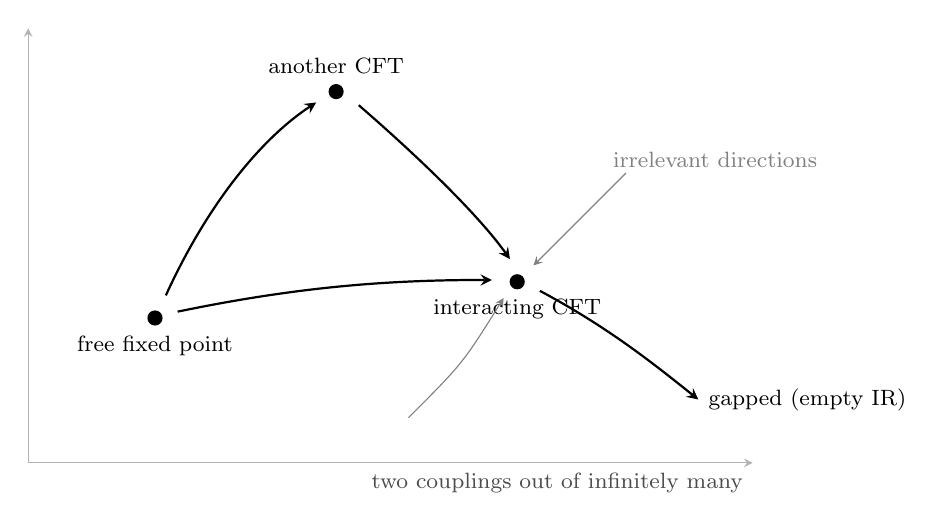
\begin{tikzpicture}[scale=1.15, >=stealth]
  % axes (suggestive)
  \draw[gray!60, ->] (-0.8,-1.4) -- (7.2,-1.4)
    node[below left, black!70]
    {\footnotesize two couplings out of infinitely many};
  \draw[gray!60, ->] (-0.8,-1.4) -- (-0.8,3.4);
  % fixed points
  \filldraw (0.6,0.2) circle (2.2pt)
    node[below=3pt] {\footnotesize free fixed point};
  \filldraw (4.6,0.6) circle (2.2pt)
    node[below=3pt] {\footnotesize interacting CFT};
  \filldraw (2.6,2.7) circle (2.2pt)
    node[above=3pt] {\footnotesize another CFT};
  % flow free -> interacting (relevant direction at free FP)
  \draw[->, thick] (0.85,0.27) .. controls (2.2,0.55) and (3.2,0.62)
    .. (4.32,0.62);
  % flow free -> other CFT
  \draw[->, thick] (0.72,0.45) .. controls (1.2,1.5) and (1.8,2.2)
    .. (2.38,2.58);
  % flow from interacting CFT to gapped
  \draw[->, thick] (4.85,0.5) .. controls (5.6,0.1) and (6.1,-0.3)
    .. (6.6,-0.7) node[right] {\footnotesize gapped (empty IR)};
  % flow from other CFT to interacting CFT
  \draw[->, thick] (2.85,2.55) .. controls (3.6,1.9) and (4.2,1.3)
    .. (4.52,0.85);
  % irrelevant flows INTO interacting CFT
  \draw[->, thin, gray] (5.8,1.8) .. controls (5.3,1.3) .. (4.78,0.78);
  \draw[->, thin, gray] (3.4,-0.9) .. controls (4.0,-0.3) .. (4.45,0.42);
  \node[gray, anchor=west] at (5.55,1.95) {\footnotesize irrelevant directions};
\end{tikzpicture}
\caption{Theory space, schematically. Points are theories; the renormalization
  group moves every non-fixed theory toward longer distances along the arrows;
  fixed points (dots) are scale-invariant theories --- CFTs --- and serve as the
  landmarks from which the rest of the space is charted. Flows out of a fixed
  point follow its relevant directions (finitely many); the gray arrows are
  irrelevant directions, along which flows converge \emph{into} a fixed point,
  producing universality.}
\label{fig:theory-space}
\end{figure}

A \vocab{fixed point} of the flow is a theory invariant under zooming out: a
scale-invariant theory. In all known unitary local examples scale invariance
comes enhanced to conformal invariance,\footnote{Proven in $d=2$
(Zamolodchikov--Polchinski), established under mild assumptions in $d=4$, and
true in every known unitary example; see Nakayama's review \texttt{1302.0884}.
We will use ``fixed point'' and ``CFT'' interchangeably, flagging the
(conjectural) gap when it matters.} so the landmarks of theory space are
\vocab{conformal field theories} --- theories with no intrinsic length scale,
looking the same at every magnification. The 3d Ising CFT of crack 3 is
precisely such a landmark, which is why it could be studied with no reference to
any flow that reaches it. It is worth pausing on how recent the consensus behind
this picture is: when Polyakov suggested at a 1970 conference that critical
points possess scale (indeed conformal) invariance, both C.~N.~Yang and T.~T.~Wu
rose to object that scale invariance in statistical mechanics was neither
mathematically nor physically justified.\footnote{The exchange is transcribed in
Rychkov \arxiv{2509.02779}, \S2 --- worth reading in full as a calibration of
how non-obvious the now-obvious can be.}

Near a fixed point, the flow linearizes, and the eigendirections sort themselves
by their behavior under zooming out: \vocab{relevant} perturbations grow (they
carry you away from the fixed point), \vocab{irrelevant} ones shrink (flows
converge back), \vocab{marginal} ones sit at the threshold. This tangent-space
structure is computable the moment you know the scaling dimensions of the fixed
point's operators. At the free (Gaussian) fixed point of a single scalar,
demanding that the kinetic action $\int d^dx\, (\partial\phi)^2$ be
dimensionless fixes
\begin{equation}
[\phi] = \frac{d-2}{2},
\qquad\text{so that}\qquad
\Big[\textstyle\int d^dx\; g_n\, \phi^n\Big] = 0
\;\;\Longrightarrow\;\;
[g_n] = d - n\,\frac{d-2}{2} .
\label{eq:power-counting}
\end{equation}
The perturbation $g_n \phi^n$ is relevant when $[g_n] > 0$, i.e.\ $n <
2d/(d-2)$: in $d = 4$ the relevant interactions stop at $\phi^3$ with $\phi^4$
marginal; in $d = 3$, at $\phi^5$ with $\phi^6$ marginal; in $d = 6$, already
$\phi^3$ is the marginal frontier; and in $d = 2$, where $[\phi] = 0$,
\emph{every} potential is relevant --- the first hint that two dimensions is a
world of its own (Part III.4). Operators with more derivatives, like
$(\partial\phi)^4$, are irrelevant in all $d \geq 2$. The pattern generalizes
beyond free fixed points --- at an interacting CFT the same counting runs on the
true scaling dimensions $\Delta$, with ``relevant'' meaning $\Delta < d$ --- and
the crucial finiteness persists: \emph{a fixed point has finitely many relevant
directions}.

That finiteness demystifies, in two sentences, the step of the standard recipe
that was always presented as a mystery. ``Renormalizable interactions'' are
exactly the relevant and marginal directions at the Gaussian fixed point: the
textbook instruction \emph{write only renormalizable terms} is the geometric
statement \emph{parametrize the flows leaving this fixed point}, and the miracle
that infinitely many possible counterterms reduce to a few measurable couplings
is no miracle --- the irrelevant directions die under the flow, so the IR
physics could never have depended on them. Conversely, every QFT used in physics
is an \vocab{effective field theory}: a local chart around a fixed point,
accurate up to corrections suppressed by powers of the distance scale, with the
irrelevant operators recording --- in a decaying, organized hierarchy --- the
memory of whatever lies upstream. The expanded version of these claims, with the
Wilson--Fisher fixed point in $d = 4 - \epsilon$ constructed as the first
nontrivial landmark, is chapter I.6's job.

The same picture finally lets us say sharply what was right about the two
traditional answers to ``what is a QFT?'', which can now be seen as two
\emph{charts} on theory space.\footnote{This comparison is drawn from Seiberg's
\emph{Thoughts About QFT}, whose slides phrase it as ``QFT in high-energy
theory'' vs.\ ``QFT in condensed-matter physics.''} The high-energy chart starts
at a fixed point and deforms by its finitely many relevant and marginal
couplings (plus, implicitly, infinitesimal irrelevant ones): a small, rigid
parametrization, anchored on a landmark --- this is the Lagrangian paradigm,
properly understood. The condensed-matter chart starts from a lattice model at
the cutoff and allows \emph{arbitrary} local couplings and arbitrary added
degrees of freedom: an enormous, floppy parametrization, in which the natural
questions are about the possible long-distance \emph{phases} and the walls
between them. The two charts overlap where both converge, and translating
between them --- which lattice models flow to which continuum landmarks, and
what data survives the trip --- is a running concern of these notes,
culminating in Part VIII.

\begin{reemark}[How much structure does theory space have?]
\label{rem:deformation-class}
It is tempting to ask global questions: is theory space connected? What are its
components? A sharp version uses the notion of a \vocab{deformation class}: two
theories are in the same class if one can interpolate between them by adding
degrees of freedom at high energy and moving along couplings, preserving the
symmetries one cares about. Seiberg has conjectured that the deformation class
is determined by precisely two pieces of data --- the global symmetry and its
't~Hooft anomalies --- both of which are exactly preserved along any flow. If
true, this gives theory space a remarkably simple coarse topology, with the
anomalies of Part II as its complete invariants. The conjecture motivates much
current work; we will be in a position to appreciate its content (and its
supersymmetric stress tests) after Part II. For now it is a preview of how
seriously the picture of this section can be taken: theory space is not a
metaphor but an object with topology, invariants, and conjectures of its own.
\end{reemark}

The rest of these notes is organized as questions about
Figure~\ref{fig:theory-space}. What structures are transported \emph{exactly}
along the flow lines, surviving from any presentation down to the deep infrared?
(Symmetries and their anomalies: Part II.) What are the fixed points, studied as
intrinsic objects? (Conformal field theory: Part III.) Which flows between
landmarks are possible, and is the flow irreversible? (Monotonicity theorems and
infrared constraints: Part IV.) How do gauge theories, the duality webs, and
the solvable supersymmetric corners populate the map? (Parts V--VII.)
When does a lattice presentation actually converge to a point of this space?
(Part VIII.) The picture is simple; what the last twenty years discovered is
how much of the subject it organizes.

\begin{exercise}[easy]
\label{exr:power-counting}
Tabulate $[\phi]$ and the relevant/marginal/irrelevant verdicts for $\phi^n$ ($n
\le 6$) and $(\partial\phi)^4$ in $d = 2, 3, 4, 6$. For a Dirac fermion (kinetic
term $\int d^dx\, i\bar\psi \slashed{\partial} \psi$), find $[\psi]$ and
classify the four-fermion interaction $(\bar\psi\psi)^2$ in $d = 2, 3, 4$. Which
famous theories live at the marginal frontier in each $d$?
\answ{$[\psi] = (d-1)/2$, so $[(\bar\psi\psi)^2] = 2(d-1)$ and the coupling has
dimension $2 - d$: marginal in $d=2$ (Thirring, Gross--Neveu), irrelevant
in $d > 2$ --- which is why the 4d Fermi theory of weak interactions
demanded a UV completion.}
\end{exercise}

\begin{exercise}[medium]
\label{exr:free-scalar-dim}
Check \eqref{eq:power-counting} against an explicit correlator: compute the
Euclidean two-point function of a free massless scalar, $\langle \phi(x) \phi(0)
\rangle = \frac{C_d}{|x|^{d-2}}$, from $\int d^dp \, \frac{e^{ip\cdot x}}{p^2}$,
and confirm that the power of $|x|$ matches $2[\phi]$ with $[\phi] = (d-2)/2$.
What replaces the power law in $d = 2$, and how does this connect to the ``every
potential is relevant'' verdict above?
\hint{In $d=2$ the integral is IR-divergent and the two-point function grows
logarithmically: $\langle\phi\phi\rangle \sim -\frac{1}{2\pi}\ln|x|$. A
dimensionless field is on the edge --- whence both the richness (vertex
operators $e^{i\alpha\phi}$ of continuously variable dimension) and the
delicacy (no SSB of continuous symmetries) of $d=2$.}
\end{exercise}

\begin{exercise}[thinker]
\label{exr:irreversibility}
Nothing in this section's picture forbids closed RG trajectories: flows that
leave a fixed point and return, or limit cycles with no fixed point at all.
Reflect on what a limit cycle would mean physically (physics periodic in the
\emph{logarithm} of the scale --- discrete scale invariance) and why one might
expect coarse-graining, which discards information, to be gradient-like instead.
This intuition is correct for unitary theories in even dimensions $\le 4$, where
it is a theorem ($c$- and $a$-theorems, Part IV.1) --- but the proofs need real
input beyond ``information is lost,'' and non-unitary counterexamples exist.
\end{exercise}

% =====================================================================
\subsection{What would count as an answer?}
\label{sec:answer}

The question in this chapter's title has, today, no complete answer --- but the
partial answers are substantial, and a reader should know the shape of the
existing attempts before chapters I.2--I.4 borrow structure from all of them.
Each of the four main axiomatic traditions formalizes a different row of the
inventory of Definition~\ref{def:inventory}.\footnote{This entire section
compresses Dedushenko's survey \arxiv{2203.08053}, which should be consulted for
precise statements and for the hundred-some references the one-line summaries
below conceal. The comparison returns, with the benefit of the whole book's
examples, in Part XII.1.}

The \vocab{Wightman axioms} (1950s) and their Euclidean counterpart, the
\vocab{Osterwalder--Schrader axioms} (1970s), axiomatize item 2: fields as
operator-valued distributions, correlators with specified analyticity,
positivity, and causality properties, and reconstruction theorems that rebuild
the Hilbert space from the correlators. Within their domain they are a complete
success --- the spin-statistics and CPT theorems are their fruits, and the
constructive program built genuine interacting examples in $d = 2, 3$ satisfying
them. Their domain, however, is local operators in flat space: gauge theories
fit awkwardly (the gauge-variant fields are not Wightman fields, and the
physical content includes the extended operators of item 4, about which the
axioms are silent), and the $(2,0)$ theory --- with no fields at all in any
classical sense --- fits not at all.

\vocab{Algebraic QFT} (Haag--Kastler, 1960s onward) drops fields in favor of
assigning to each spacetime \emph{region} the algebra of observables measurable
inside it, with compatibility under inclusion and commutativity at spacelike
separation. It is the formulation in which the deep structural results about
quantum information in field theory live --- the type classification of local
algebras, Tomita--Takesaki modular theory, the Reeh--Schlieder theorem --- and
Part X of these notes is, in effect, its payoff. Its classic limitation is
mirror to Wightman's: theories are easy to axiomatize but hard to construct, and
topological sectors (instantons, again the extended operators) strain the
axioms' locality assumptions in ways that current research is still sorting out.

\vocab{Functorial QFT} (Atiyah--Segal, late 1980s; Kontsevich--Segal for the
non-topological case) axiomatizes items 1 and 3 directly: a QFT is an assignment
of Hilbert spaces to space-slices and of evolution maps to spacetime cobordisms
between them, compatible with gluing --- the path integral's cutting-and-sewing
behavior elevated to the definition. For \emph{topological} theories this
definition is not merely rigorous but spectacularly classifiable, and it is the
natural home of every ``assign data to manifolds'' instinct in this chapter
(chapter I.4 is built on it). For theories with metric dependence it faces real
open problems: which complex metrics are allowable (the Kontsevich--Segal
criterion \arxiv{2105.10161}, chapter I.4's modern answer to ``what is Wick
rotation?''), and how to accommodate the scheme ambiguities of genuine QFTs,
where the partition function on a curved background is not a number but a
number-up-to-local-counterterms.

And the \vocab{lattice} tradition --- physics' working definition --- defines a
theory as the continuum limit of a regularized system, with constructive field
theory as its rigorous wing. Its strengths and its audit findings (triviality;
exotic limits) have already appeared in this chapter, and Part VIII is devoted
to it.

\medskip

\noin Four traditions, four fragments --- and the honest summary is that none
captures class $\mathcal{S}$, large-$N$ limits, \emph{and} fracton models
simultaneously, while the developments of Parts II--XI (symmetry
categories as part of a theory's identity; defects on equal footing with
local operators) are only beginning to be reflected in any of them.
Dedushenko's verdict stands: \emph{formulating a complete definition of
QFT is an outstanding open problem}, of equal interest to physics and
mathematics. These notes take the working position already staked out in
this chapter --- the inventory, locality, and consistency, used
opportunistically through whatever presentation converges --- and treat
the missing definition not as an embarrassment but as the subject's
standing research frontier, revisited with better equipment in Part XII.1.

\begin{nnote}[What these notes assume]
Operationally, the chapters ahead assume of every theory: unitarity (reflection
positivity in Euclidean signature), a local stress tensor, cluster
decomposition, and --- in flat space --- Poincar\'e invariance, flagging
explicitly each time one of these is relaxed (non-unitary fixed points, little
strings, fractons, theories without stress tensors all make scheduled
appearances). When an argument depends on an unproven structural assumption ---
existence of a continuum limit, convergence of an OPE beyond CFT, enhancement of
scale to conformal invariance --- the dependence is stated where it occurs.
\end{nnote}

% =====================================================================
\subsection*{Chapter exercises}

\begin{exercise}[classic]
\label{exr:field-redef}
(Two Lagrangians, one theory, in $d=0$.) In the integral \eqref{eq:zerod-Z},
change variables $\phi = \psi + c\,\psi^3$ for small constant $c$. Show that the
resulting ``theory of $\psi$'' has a different-looking action --- new
interaction vertices $\psi^4, \psi^6, \dots$ with $c$-dependent couplings, plus
a vertex from the Jacobian --- yet \emph{identical} partition function, and
(after matching sources) identical correlators of the original operator.
Conclude that coupling constants of presentations are not, in general,
observables. Which combinations of the new couplings are invariant?
\hint{The Jacobian $d\phi = (1 + 3c\psi^2)\,d\psi$ exponentiates into the action
as $-\ln(1+3c\psi^2)$. This freedom of field redefinition is the $d=0$
shadow of the equivalence theorem; ``the theory'' is the equivalence
class.}
\end{exercise}

\begin{exercise}[medium]
\label{exr:large-order}
(Large orders from the complex saddle.) Represent the coefficients of
Example~\ref{ex:zero-d} as $a_n = \oint \frac{d\lambda}{2\pi i}\,
\frac{Z(\lambda)}{\lambda^{n+1}}$ and evaluate the large-$n$ behavior by saddle
point: the contour is pushed onto the negative-$\lambda$ cut, where the
discontinuity of $Z$ is computed by the instanton saddle $\phi_\ast^2 =
-6/\lambda$ with action $-3/2\lambda$. Recover the growth $|a_n| \sim
n!\,(2/3)^n$ of \eqref{eq:an-asymptotic}, including the power of $n$ in the
prefactor if you are feeling thorough.
\hint{$\mathrm{Disc}\, Z(-|\lambda|) \propto e^{-3/2|\lambda|}/\sqrt{|\lambda|}$
from the Gaussian integral over the unstable direction at the saddle. Then
$a_n \approx \frac{1}{\pi}\int_0^\infty
\frac{d|\lambda|}{|\lambda|^{n+1}}\,\mathrm{Im}\,Z(-|\lambda|)$ is
dominated by $|\lambda| \sim 3/2n$. This dispersive route from instantons
to large orders is the $d=0$ version of the Lipatov/Bender--Wu analysis.}
\end{exercise}

\begin{exercise}[medium]
\label{exr:circle-correlator}
(A correlator on the circle.) For the particle on a circle at general $\theta$,
compute the Euclidean two-point function $\langle e^{iq(\tau)}\, e^{-iq(0)}
\rangle_\beta$ by inserting energy eigenstates, and examine its $\beta \to
\infty$ limit. Show that the answer decays exponentially in $\tau$ with rate set
by the gap, in parallel with \eqref{eq:ising-correlator} --- except at $\theta =
\pi$, where the degeneracy makes part of the correlator \emph{persist} at
infinite separation. Interpret the persistent piece as spontaneous breaking of
the $C$ symmetry between the two ground states, in the only way quantum
mechanics permits: exact degeneracy.
\hint{$e^{iq}\ket{n} = \ket{n+1}$, so the correlator is $\frac{1}{Z}\sum_n
e^{-(\beta - \tau) E_n - \tau E_{n+1}}$. At $\theta = \pi$, the $n = 0$
term contributes $e^{-\beta E_0}$ with \emph{no} $\tau$-dependence in the
exponent's leading piece, since $E_0 = E_1$.}
\end{exercise}

\begin{exercise}[thinker]
\label{exr:axioms-vs-cracks}
Each of the four cracks of Section~\ref{sec:four-cracks} embarrasses at least
one axiom system of Section~\ref{sec:answer}. Match them: which axioms could in
principle accommodate the $(2,0)$ theory but cannot construct it? Which
formalize a duality like \eqref{eq:particle-vortex} as an exact statement, and
which cannot even state it? Which tradition does the triviality theorem
vindicate, and which does it humble? Use Dedushenko \arxiv{2203.08053} \S3 as a
referee for your answers.
\end{exercise}

\begin{exercise}[thinker]
\label{exr:two-theories-same-correlators}
Idea~\ref{idea:observables} says a theory is its observables. Here is a stress
test you can hold in mind through chapter I.3: could two \emph{distinct}
theories have identical correlation functions of all \emph{local} operators on
$\reals^d$, differing only in their extended operators or in their partition
functions on topologically nontrivial spacetimes? (No proof expected --- but
formulate precisely what data would have to differ, and what experiment, in a
finite-size sample, would tell the two theories apart.) The answer is yes, the
canonical examples being gauge theories with the same algebra and different
global structure, e.g.\ $SU(2)$ vs.\ $SO(3)$ Yang--Mills; this is the content of
``reading between the lines'' \arxiv{1305.0318}, and the reason item 4 sits in
Definition~\ref{def:inventory}.
\end{exercise}

% =====================================================================
\subsection*{Reading}

\begin{description}
\item[Dedushenko, \emph{The Quest to Define QFT}, \arxiv{2203.08053}.] The
survey behind Section~\ref{sec:answer}: a short overview of every axiom
system, with its successes and limitations, and a bibliography that leads to
the original literature. Read \S\S1, 3 now and \S2 as reference.
\item[Rychkov \arxiv{2509.02779}.] \emph{Conformal bootstrap: from Polyakov to
our times}. The history that makes the modern viewpoint feel inevitable rather
than fashionable: the 1970 Kyiv exchange, Polyakov's 1974 manifesto, and the
road to the Ising island. Sections 2--5 complement this chapter; the rest seeds
Part III.
\item[Seiberg, \emph{Thoughts About Quantum Field Theory} (IAS).] The
reorganization manifesto in slide form: theories without Lagrangians,
deformation classes, symmetries-and-anomalies as the invariants of theory space.
Twenty minutes that frame the whole book.
\item[Gaiotto--Kapustin--Komargodski--Seiberg, \arxiv{1703.00501}, Appendix D.]
The particle on a circle, done as a warm-up for Yang--Mills at $\theta = \pi$
--- the source for Example~\ref{ex:particle-circle} and the bridge to Parts II.7
and V.3.
\item[Seiberg--Senthil--Wang--Witten, \arxiv{1606.01989}, \S1.] What duality
means, by example; the duality web behind crack 2.
\item[Aizenman--Duminil-Copin, \arxiv{1912.07973}, \S1.] The triviality theorem.
The introduction is readable by physicists and states exactly what is and is not
proven.
\item[Poland--Rychkov--Vichi, \arxiv{1805.04405}, \S1.] The data-centric view of
CFT from the practitioners; the source of the numbers in \eqref{eq:ising-dims}.
\item[Books (for the shelf, not the week):] Glimm--Jaffe, \emph{Quantum Physics:
A Functional Integral Point of View} --- what ``constructing a QFT'' means when
done in earnest; Weinberg, \emph{The Quantum Theory of Fields I}, ch.\ 1 --- the
historical case that QFT was forced on us, the perfect foil for this chapter's
question.
\end{description}
